\documentclass[headsepline=true, footsepline=true]{scrartcl}

\usepackage{tutorial}

%% ==============================================================
\title{Separates Deployment von Produktdaten}
\author{Cornelius Dirmeier}
\setcopyright{
\includegraphics[height=10pt]{./pics/FaktorZehn-ORG.png}}
%% ==============================================================

\begin{document}

\maketitle

\section{Einleitung}

Faktor-IPS verwaltet Produktdaten während der Produktentwicklung in XML Dateien.
Zur Laufzeit wird bisher (Version 2.5. und frühere Versionen) ebenfalls mit XML
Dateien gearbeitet. Genau genommen muss man von XML-Ressourcen sprechen, da die
einzelnen XML-Dateien meist in Bibliotheken (z.B. JAR-Dateien) zusammengefasst
werden. Um die Produktdaten zu laden müssen sie zur Laufzeit im Classpath der
Applikation verfügbar sein, entweder als einzelne Dateien oder in Form von
Bibliotheken. Innerhalb einer Applikation kann auf die Produktdaten über ein
Runtime Repository (z.B. $ClassloaderRuntimeRepository$) zugegriffen werden.

\begin{figure}[htb] \centering
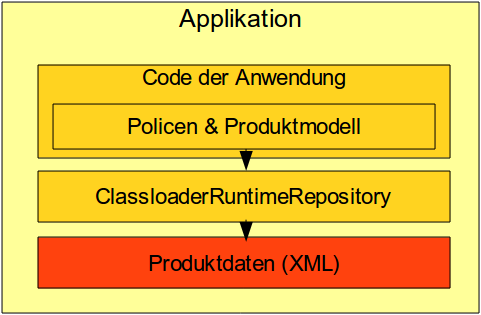
\includegraphics[width=8cm]{./pics/old_architecture.png}
\caption{Bisher wurden Programmcode und Produktdaten in einer gemeinsamen
Applikation ausgeliefert}
\label{old_architecture}
\end{figure}

Da sowohl Programmcode als auch Produktdaten als Dateien vorliegen, können sie
zusammen in einem Werkzeug wie CVS oder Subversion gespeichert werden. Eine
fertige Version von Programmcode und Produktdaten wird dann in eine Zielumgebung
transportiert. Im JavaEE Umfeld wird dazu ein Enterprise Archive (EAR) bzw. ein
Web Application Archive (WAR) erzeugt.

Werden die Produktdaten verändert oder erweitert muss dieses Archiv ausgetauscht
werden. Da Produktdaten und Programmcode eine Einheit bilden, muss auch der
Programmcode neu ausgeliefert werden.

Ziel des separaten Deployments von Produktdaten ist es, bei einer Änderung der
Produktdaten nur die XML-Ressourcen auszutauschen ohne den Programmcode neu
ausliefern zu müssen. Die Probleme, die dabei auftretenden Herausforderungen und
die daraus entwickelten Lösungen werden in diesem Dokument vorgestellt.

\section{Herausforderungen}

\subsection{Runtime Repository}

Für den Zugriff auf die Produktdaten steht in Faktor-IPS zur Laufzeit das
Interface $IRuntimeRepository$ zur Verfügung. Wie bereits einleitend
erwähnt wurde bisher meist die Implementierung
$ClassloaderRuntimeRepository$ verwendet. Dieses lädt die Produktdaten über den
Klassenpfad als Ressourcen.

Um die Produktdaten unabhängig vom Programmcode zu halten muss zunächst ein
Repository entwickelt werden, dass die Produktdaten unabhängig vom Klassenpfad
der Applikation laden kann. Die hier vorgestellte Lösung greift dazu auf einen
separaten Service (EJB 3.0 Stateless Session Bean) zu; die Verwendung einer
Datenbank soll aber ohne großen Aufwand implementierbar sein.

\subsection{Ausführen von Formeln}

In Faktor-IPS ist es möglich Formeln in einer einfachen Formelsprache in einem
Produktbaustein einzugeben. In den Modellklassen wird lediglich die Signatur der
Formel festgelegt, die Berechnungsvorschriften liegen in den Produktdaten. Um
diese Formeln zur Laufzeit effizient auszuführen werden sie vom
Faktor-IPS-Builder in Java-Code übersetzt.

Bisher wurde dazu für jeden Produktbaustein\footnote{Genau genommen werden
Formel für eine Anpassungsstufe festgelegt, dies würde jedoch die Beschreibung
unnötig verkomplizieren} eine Subklasse erzeugt, in der die Methode der Formel
überschrieben wurde. Das Runtime Repository war so aufgebaut, dass es jeweils die
korrekte Implementierung zu einem Produktbaustein lud.

\begin{figure}[htb] \centering
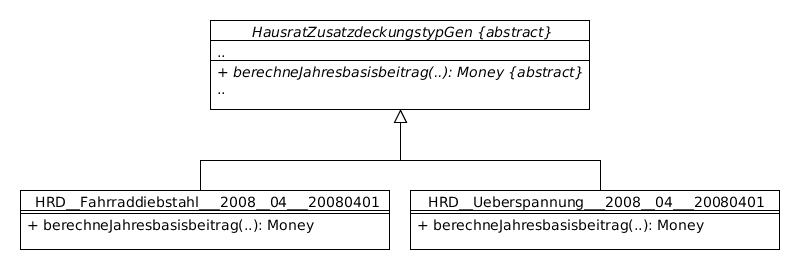
\includegraphics[width=13cm]{./pics/subclassing.png}
\caption{Für jeden Produktbaustein wird eine Subclass angelegt, in der die
übersetzte Formel implementiert ist.}
\label{subclassing}
\end{figure}

Werden nun die Produktdaten durch einen separaten Service abgerufen, 

Beim separaten Ausliefern von Produktdaten entsteht dabei das Problem, dass mit
den Produktdaten nicht nur XML-Ressourcen sondern auch Programmcode ausgetauscht
werden muss. Der normale Classloading Mechanismus von Java sieht ein Austauschen
von Bytecode zur Laufzeit nicht vor. Da im Java EE Umfeld von vielen Application
Servern der Classloading Mechanismus beeinflusst wird, ist es nicht sinnvoll
hierfür eigene Lösungen aufzubauen.

Es musste also Teil des separaten Deployments sein, die Formeln
zur Laufzeit zu interpretieren um die Produktdaten frei von Programmcode zu
halten.

\subsection{Hot Deployment und Caching}
\label{hot_deployment}

Eine weitere Herausforderung stellt das Hot Deployment dar. Es soll möglich
sein, die Produktdaten bei laufendem Betrieb auszutauschen.

Um die Performance der Anwendung beizubehalten, müssen Produktdaten außerdem
gecached werden. Die bisherigen Implementierungen von $IRuntimeRepository$
enthalten dazu bereits etablierte Lösungen. Eine Aufgabe des neuen Repositories
ist es, eine Strategie zu realisieren, damit bei einer neuen Auslieferung der
Produktdaten die Caches gelöscht werden.

Ein weiteres Problem des Hot Deployments ergibt sich durch
Clients\footnote{Als Client bezeichnen wir den Benutzer des Services}, die aktuell Produktdaten abrufen. Ein Client ruft
üblicherweise während der Bearbeitung einer Anfrage mehrmals Daten vom
Repository ab. Werden die Produktdaten zwischen zwei Abfragen ausgetauscht, 
muss der Client entsprechend informiert werden.

Hat ein Client festgestellt, dass sich die Produktdaten geändert haben, muss er
dem Runtime Repository melden, dass er ab sofort mit den neuen Produktdaten
arbeiten möchte. Ein anderer Client, der bisher nichts von dem Austausch der
Produktdaten mitbekommen hat muss jedoch beim nächsten Aufruf ebenfalls
informiert werden. Hier ist eine geeignete Lösung zu finden, die effizient
und sicher viele Clients bedienen kann.

\section{Lösungen}

\subsection{Architektur der Services}

Wie bereits in der Anleitung erwähnt, betrachten wir die Auslieferung in einem
Java EE Umfeld. Die verschiedenen Programmteile werden als Services
implementiert und in einem EAR ausgeliefert.

Wie bisher wird der Programmcode mit den Modellklassen in einem Archiv gekapselt.
Anstatt des $ClassloaderRuntimeRepositories$ wird eine neue Implementierung von
$IRuntimeRepository$ verwendet: das $ProductDataProviderRuntimeRepository$.
Dieses ruft zum Laden der Produktdaten einen zweiten Service auf, den
$ProductDataService$. Im Archiv des $ProductDataService$s sind die Produktdaten
weiterhin als XML-Ressourcen enthalten und können vom Service über den Classpath
geladen werden.

\begin{figure}[htb] \centering
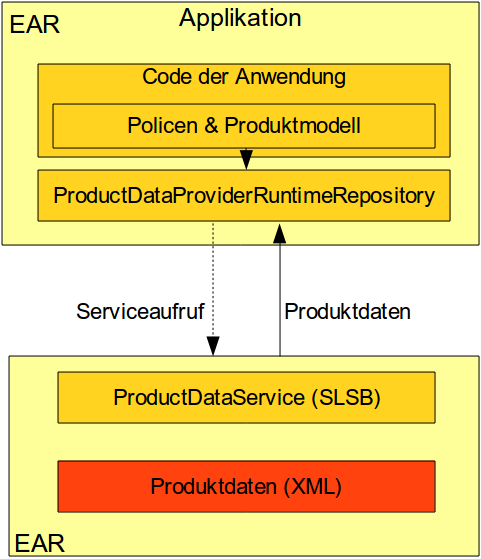
\includegraphics[width=8cm]{./pics/service_architecture.png}
\caption{Die Produktdaten werden in einem separaten Service ausgeliefert der
vom Runtime Repository verwendet wird.}
\label{service_architecture}
\end{figure}

Der $ProductDataService$ wird als Stateless Session Bean (SLSB) implementiert.
Die Produktdaten werden als XML-Ressourcen geladen, der Inhalt wird an das
Runtime Repository übergeben. Die Instantiierung findet weiterhin im Runtime
Repository statt.

\subsection{Interpretation von Formeln}

Um die Formeln nicht in Subklassen zu implementieren muss ein Mechanismus zum
Interpretieren des Formel-Codes geschaffen werden. Da das Compilieren der
Formeln in Java-Code bereits existiert, war die einfachste Möglichkeit diesen
Mechanismus weiter zu verwenden. Anstatt den Java-Code in Subklassen zu
schreiben, kann er in Zukunft auch in das XML der Produktbausteine geschrieben
werden. Der Java-Codes wird zur Laufzeit von
Groovy\footnote{http://groovy.codehaus.org/} ausgeführt. Die Produktdaten
enthalten dadurch keinen Programmcode und sind unabhängig vom Classloader der Applikation.

\subsection{Cachingstrategie}

Zum Cachen der bereits geladenen Produktdaten wird wie bisher ein $SoftRefence$
Cache verwendet. Die Spezielle Implementierung $ExpirableSoftReferenceCache$
erhält im Konstruktor einen $IModificationChecker$ und merkt sich die aktuelle
Version der Produktdaten. Vor jeder Cacheanfrage wird der
Modification Checker abgefragt, ob die gespeicherte Version noch aktuell ist.
Ist die Version abgelaufen, wird der Cache geleert und die neue Version
gespeichert.


\subsection{Umgang mit mehreren Clients}

Wie in Abschnitt \ref{hot_deployment} beschrieben, muss bei mehreren Clients
darauf geachtet werden, dass jeder Client rechtzeitig über veränderte
Produktdaten informiert wird. Zunächst wird das grundsätzliche
Verhalten des Repositorys bei veränderten Produktdaten erläutert:

Um das $IRuntimeRepository$ Interface für bestehende Anwendungen nicht
anzupassen, wird bei veränderten Produktdaten vom Runtime Repository eine
RuntimeException ($DataModifiedRuntimeException$) geworfen. Wenn ein Client diese
Exception erhält, muss er seine Abfrage abbrechen um nicht mit korrupten
Produktdaten weiter zu arbeiten. Vor seinem nächsten Aufruf muss er die Methode
$reload()$ am Repository aufrufen.

Üblicherweise werden in einer Anwendung mehrere Clients parallel auf einem
Runtime Repository arbeiten. Durch den gemeinsam verwendeten Cache wird die
Performance gesteigert und Ressourcen geschont. Mit der Möglichkeit des
getrennten Prouktdatendeployments muss jedoch jeder Client über Änderungen der
Produktdaten informiert werden. In dem bisher beschriebenen Ansatz kann dies
nicht garantiert werden, da das Runtime Repository ohne Fehler die neuen
Produktdaten liefert, sobald ein Client die $reload()$ Methode aufgerufen hat.






\subsection{Architektur des ProductDataProviderRuntimeRepositorys}



Der Produktdatenservice ist ein Stateless
Session Bean (SLSB), welches die Produktdaten zur Verfügung stellt. Die
Produktdaten sind zusammen mit dem SLSB in einem eigenen EAR gebundelt. Dadurch
können die Produktdaten durch Deployment einer neuen Version des
ProduktDataService-EARs ausgetauscht werden. Der Produktdatenservice kann die
Produktdaten auf zwei Arten zur Verfügung stellen: 1.XML Das Erzeugen der
Instanzen der Modellklassen erfolgt dann im RuntimeRepository der eigentlichen
Applikation. 2.Instanzen der Modellklassen (Produktbausteine, Tabellen, Enums).
Die Produktklassen des Modells würden in diesem Fall auch als Transportobjekte
eingesetzt werden und müssten alle Serialisierbar sein.

Formeln Neben reinen Produktdaten können in Faktor-IPS in den Produktbausteinen
auch Formeln zur Berechnung hinterlegt werden. Diese Formeln werden bisher
(wiederum Version 2.5. und frühere Versionen) zur Entwicklungszeit bzw. beim
„Build“ in Java Sourcecode übersetzt. Zur Laufzeit besteht die Produktinformation
damit aus XML-Ressourcen und, falls Formeln verwendet werden, Java-Klassen. Die
Unterstützung von Formeln stellt eine besondere Herausforderung dar. Wieso? Eine
Java-Klasse, die einmal von der virtuellen Maschine geladen wurde, kann nicht
mehr verändert oder ausgetauscht werden. Wird nun also eine Formel geändert,
beispielsweise weil sie fehlerhaft war, dann müsste man aber genau die alte
Formelklasse durch die neue Formelklasse ersetzen. Eine Möglichkeit gibt es dies
umzusetzen. Genau genommen existiert eine Java-Klasse nicht einmal pro JVM,
sondern einmal pro ClassLoader. Man könnte die Formelklassen also über einen
eigenen ClassLoader laden und bei Änderungen einen neuen ClassLoader verwenden.
Da ApplicationServer allerdings selber massiv Gebrauch von dieser Möglichkeit
machen, ist die Erzeugung eigener ClassLoader im EJB Umfeld nicht gestattet. Da
die Möglichkeit, die Formeln zur Entwicklungs/Buildzeit in Java-Sourcecode zu
übersetzen damit ausfällt, müssen die Formeln zur Laufzeit interpretiert werden.
Hierzu gibt es zwei prinzipielle Varianten: 1.Entwickeln eines eigenen
Interpreters für die Formelsprache 2.Übersetzen der Formeln zur Laufzeit in Java
Sourcecode und Interpretation des Java-Sourcecodes. Da es bereits mehrere
ausgereifte Möglichkeiten gibt, Java Sourcecode zu interpretieren, soll kein
eigener Formelinterpreter geschrieben werden, sondern eine vorhandene Möglichkeit
zur Interpretation von Java Sourcecode eingesetzt werden. In Frage kommen hier
Java BeanShell und Groovy. Java BeanShell1 BeanShell ist ein Interpreter für
Java. In der Faktor-IPS Entwicklung wird er von Beginn an für die Ausführung der
Junit-Testfälle verwendet. Standardisierung wird über den JSR-274 betrieben. Mit
Aufkommen immer neuer Skriptsprachen für die JVM ist es aber sehr ruhig um
BeanShell geworden. Groovy2 Eine dynamische Sprache für die JVM. Eine Eigenschaft
von Groovy ist, dass Java Sourcecode auch gültiger Groovy-Sourcecode ist. Groovy
auch zudem als Scriptengine im Sinne des JSR 223 (ab Java 6) verwendet werden.
Wir favorisieren Groovy zur Interpretation der Formeln. Die Gründe hierfür sind:
Erste Performance-Messungen haben ergeben, dass die Ausführung der Formeln mit
Groovy wesentlich performanter ist als mit Java BeanShell. Zudem gibt es eine
sehr aktive Groovy Community während bei der BeanShell Entwicklung in letzter
Zeit wenig Fortschritt zu erkennen ist. Caching \& Hot Deployment Um die
Performance der Anwendung nicht zu verschlechtern, müssen die
Produktinformationen gecached werden. Da das Parsen von XML eine relativ teure
Operation ist, reicht es nicht aus, die XML-Daten lediglich innerhalb des
Produktdatenservices zu cachen. Statt dessen müssen, wie bisher auch, die
Instanzen (Produktbausteine, Tabellen) im RuntimeRepository der Applikation
gecached werden. Damit benötigt man aber ein Konzept, um diesen Cache zu leeren,
wenn die Produktdaten geändert wurden, die der Produktdatenservice zur Verfügung
stellt. Zudem muss sichergestellt werden, dass innerhalb einer Verarbeitung
innerhalb der Applikation mit konsistenten Produktdaten gearbeitet wird.
Detaillierung siehe Foliensatz.

\end{document}
